\documentclass[../master]{subfiles}

%\graphicspath{{../eps/}}

\begin{document}

\chapter{中性子検出器}
\section{液体シンチレータ}
${}^{12}\mathrm{C}(\mathrm{n},\mathrm{n}'){}^{12}\mathrm{C}^{\text{Hoyle}}$反応の断面積の測定には
MAIKo TPC に入射した中性子の数を測定する必要がある.
中性子は電荷をもっておらず検出器中でエネルギーを落とさないため,
直接検出することができない.
そのため,中性子と散乱した検出器中の陽子を検出することによって間接的に中性子を検出する.
より効率的に中性子と陽子が散乱するように,中性子検出器には水素が多く含まれる有機シンチレータが用いられる.
OKTAVIAN での測定ではNE213/BC501 液体シンチレータを用いる.
図\ref{fig::neutron_detector}に中性子検出器の模式図を示す.
\begin{figure}
  \centering
  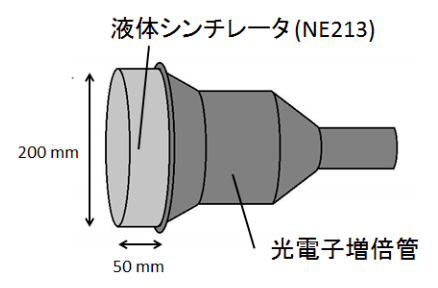
\includegraphics[clip, width=0.6\columnwidth]{pic/neutron_detector.png}
  \caption{中性子検出器の模式図.}
  \label{fig::neutron_detector}
\end{figure}
液体シンチレータの有感体積は,直径\SI{200}{\milli\metre},厚さ\SI{50}{\milli\metre}の円柱である.
容器はアルミニウム製であり,シンチレーション光の反射率を高めるために酸化マグネシウムで容器の内側はコーティングされている.
シンチレーション光は光電子増倍管で電気信号に変換されて読み出される.

\section{n-$\gamma$弁別}
液体シンチレータを用いた測定では中性子だけでなく背景$\gamma$線も検出される.
そのため,中性子と$\gamma$線の識別が必要となる.
中性子と$\gamma$線では液体シンチレータの発光の波形が異なることが知られている.
図\ref{fig::pulse_shape_n_gamma}に中性子と$\gamma$線の波形の違いの模式図を示す.
\begin{figure}
  \centering
  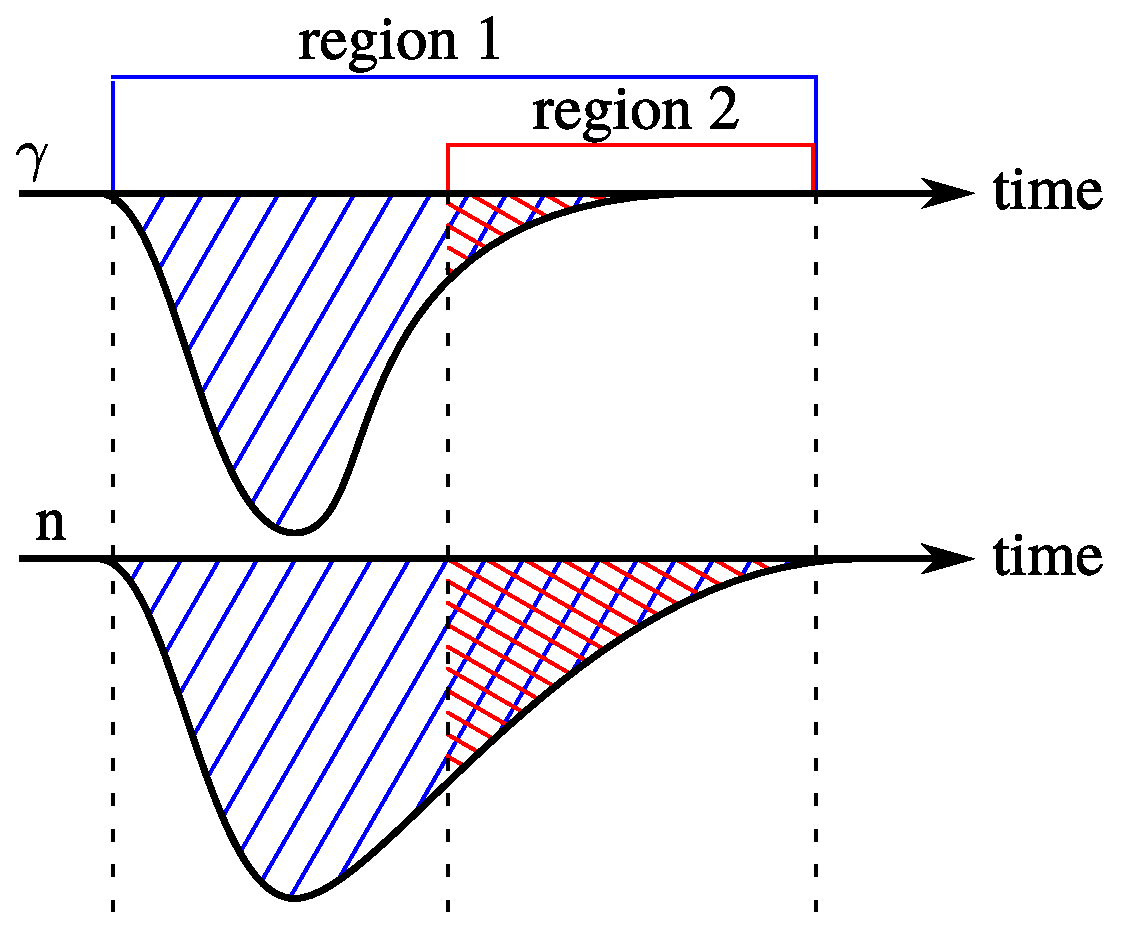
\includegraphics[clip, width=0.8\columnwidth]{integration_region.eps}
  \caption[液体シンチレータから得られる中性子および$\gamma$線の波形の違いと2つの積分区間.]
          {液体シンチレータから得られる中性子および$\gamma$線の波形の違いと2つの積分区間.
            全体を覆う区間 (region 1) とテール部分を覆う区間 (region 2) とにより波形を識別する.
          }
  \label{fig::pulse_shape_n_gamma} 
\end{figure}
中性子の方がテールが長く引いた波形となる.
図\ref{fig::pulse_shape_n_gamma}に示すように,
波形全体を覆う区間 (region 1) とテール部分を覆う区間 (region 2) の2つの積分区間を用いて波形を積分することで,
中性子と$\gamma$線とを区別する.

中性子検出器から得られる信号はCAEN V1742 を用いて取得した.
CAEN V1742 は入力信号の波形をそのまま取得することができるモジュールである.
信号の取得周波数は\SI{5}{\giga\hertz} から \SI{750}{\mega\hertz} である.
CAEN V1742 で取得した波形の1例を図\ref{fig::waveform_V1742}に示す.
\begin{figure}
  \centering
  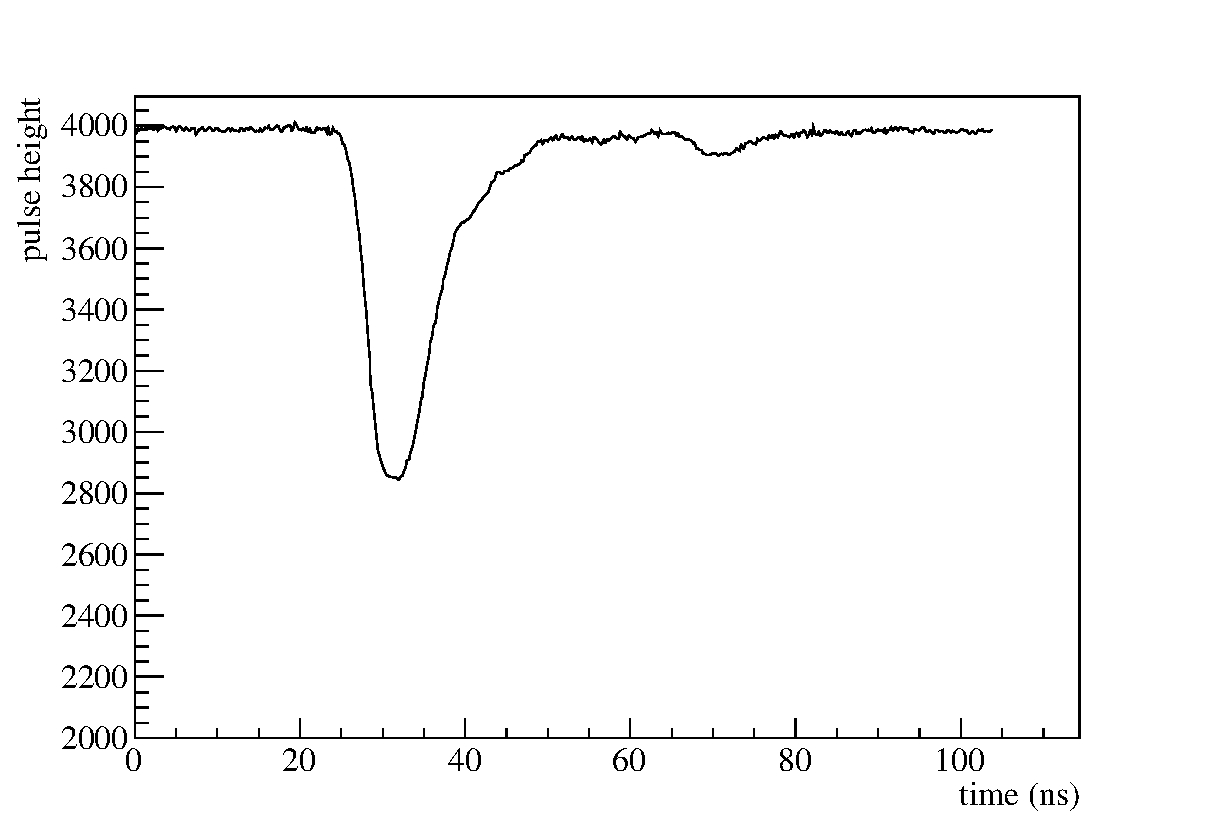
\includegraphics[clip, width=0.8\columnwidth]{waveform_V1742.eps}
  \caption{V1742で取得した波形の1例.}
  \label{fig::waveform_V1742}
\end{figure}
図\ref{fig::waveform_V1742}はAmBe 中性子線源を用いて測定をした.
取得周波数は\SI{5}{\giga\hertz}である.

V1742 によって取得した波形のピーク位置に対して
\SI{-15}{}--\SI{45}{\nano\second} (region 1) と\SI{10}{}--\SI{45}{\nano\second} (region 2) の2つの区間で波形を積分した.
AmBe 中性子線源で取得したregion 1 とregion 2 の相関を図\ref{fig::n_gamma_correlation}に示す.
\begin{figure}
  \centering
  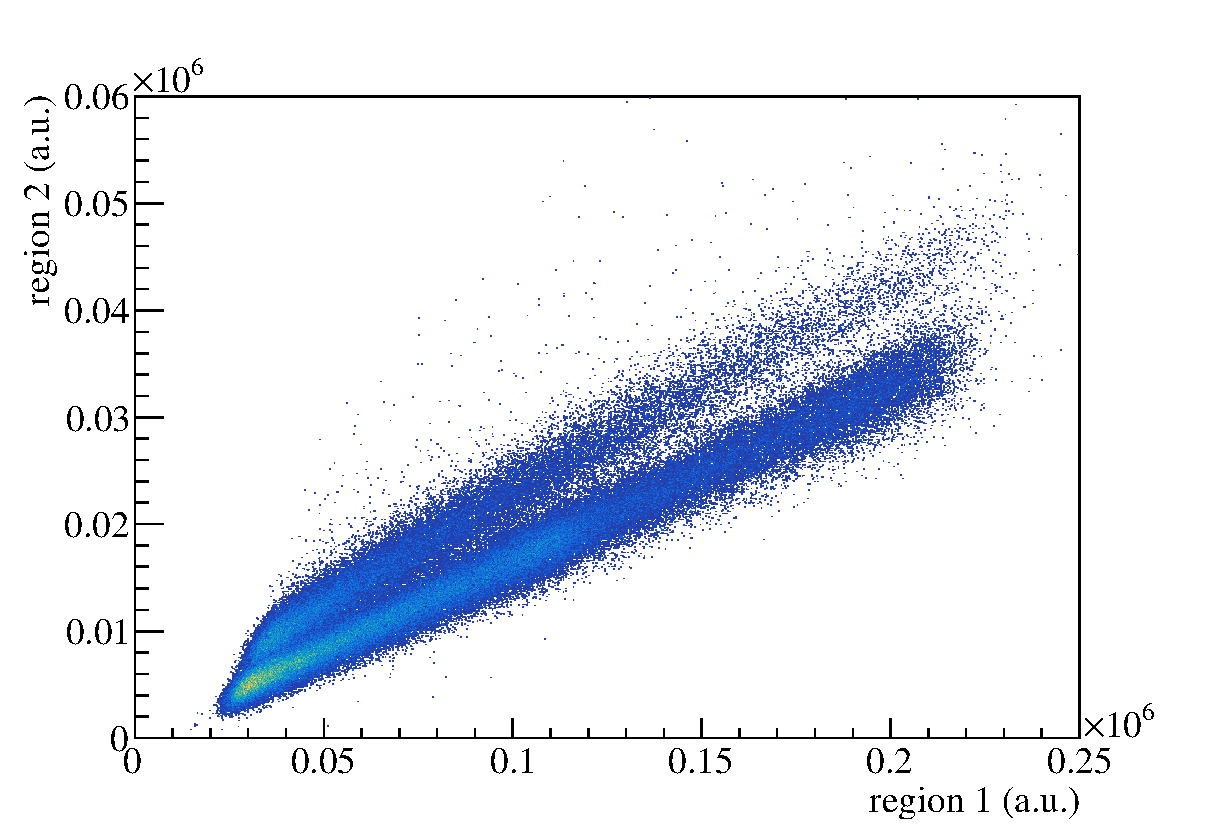
\includegraphics[clip, width=0.8\columnwidth]{n_gamma_corr.eps}
  \caption[region 1 とregion 2 と2つの区間での積分値の相関.]
          {region 1 とregion 2 と2つの区間での積分値の相関.
            AmBe 中性子線源を用いて測定した.
          信号がV1742 のダイナミックレンジを超えたものはカットしている.}
  \label{fig::n_gamma_correlation}
\end{figure}

\section{キャリブレーション}
\section{SCINFUL-CG による中性子の検出効率}
検出器中に入射した中性子が他の粒子と反応しない場合は検出されない.
そのため、検出器に入射した中性子の絶対数を求めるためには検出効率を知る必要がある.
液体シンチレータの検出効率を求める計算コードにSCINFUL-CG~\cite{scinful-cg}がある.

\end{document}
